\subsection{Prueba unitaria}
Las primera prueba unitaria fue sobre los actores. En esta sección se describe 
como se realiza la prueba y como se solucionan los errores encontrados a partir 
de ella. 
\subsubsection{Objetivo de la prueba}
Verificar el funcionamiento lógico de los componentes del nivel y definir los 
valores a algunos atributos para el funcionamiento correcto de algunos actores. 
\subsubsection{Herramientas utilizadas durante la prueba}
\textit{Unity.}
\subsubsection{Aplicación de la prueba}
Para esta prueba se evaluá el comportamiento de los actores antes de su 
integración a los niveles y como estos interactúan con el jugador. Unity permite 
ver los valores que adquieren los atributos durante su ejecución, ver figura 
\ref{fig:Debug01}. Así que para esta prueba basta con ejecutar la escena 
base y observar como responden los actores.
\\
\par
Primeramente se revisa que los enemigos y las plataformas sigan sus patrones de 
movimiento definidos. Después se verifica que los enemigos, obstáculos e ítems 
afecten la cantidad de vida del jugador y en algunos casos su cantidad de 
\textit{tonalli}. En el caso de los jefes se verifica que sus ataques no se vean 
interrumpidos por nuevos ataques de la maquina de estados. En el caso particular 
de obstáculos como \textit{WindCreator} se definen los intervalos de tiempo 
para su correcto funcionamiento. 

		\begin{figure}[h]
    			\centering
    			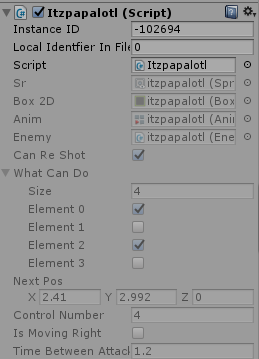
\includegraphics[width=0.2\textwidth]{04ResultadosObetnidos/imagenes/enemyPruebas01.png}
    			\caption{Unity permite ver los valores de los tributos de las clases en ejecución.}
    			\label{fig:Debug01}
		\end{figure}
		
\subsubsection{Conclusiones de la prueba}
En esta prueba se observan diferentes problemas en el comportamiento de los actores 
que se solucionan, a continuación se mencionan los errores encontrados y como se 
solucionaron:
        \begin{itemize}
                \item El marcador se actualiza al doble cuando el jugador cae 
                sobre un objeto coleccionable: Este error resulta producto de 
                utilizar un \textit{GameObject} auxiliar para la detección de las 
                colisiones del suelo. El error se soluciona facilmente al agregar 
                un componente de tipo rigidbody 2D al \textit{GameObject} auxiliar 
                para la detección de las colisiones del suelo.
                \item Los ítems restauran el doble de vida cuando el jugador cae 
                sobre ellos: Este error es generado por las mismas causas que el 
                de los objetos coleccionables así que al solucionar el de los 
                objetos collecionables se soluciona éste.
                \item Los ataque de los jefes generados por corrutinas se 
                empalman con otros ataques o interrumpen los que ya se estan 
                ejecutando: Esto se soluciona al detener todas la corrutinas generadas 
                por el jefe cuando se ejecuta un ataque.
        \end{itemize}
